\documentclass[a4paper,11pt]{jsarticle}

% 数式
\usepackage{amsmath,amsfonts}
\usepackage{amsthm}
\usepackage{bm}
\usepackage{mathtools}

% 表
\usepackage[utf8]{inputenc}
\usepackage{diagbox} % 斜線付きセルを作成するために必要
\usepackage{booktabs} % 表の罫線を美しくするために必要
\usepackage{hhline} % 水平罫線を制御するために必要

% 画像
\usepackage[dvipdfmx]{graphicx}
\usepackage{ascmac}
\usepackage{physics}
\usepackage{float} % 追加

% 図
\usepackage[dvipdfmx]{graphicx}
\usepackage{tikz} %図を描く
\usetikzlibrary{positioning, intersections, calc, arrows.meta,math} %tikzのlibrary

% ハイパーリンク
\usepackage[dvipdfm,
  colorlinks=false,
  bookmarks=true,
  bookmarksnumbered=false,
  pdfborder={0 0 0},
  bookmarkstype=toc]{hyperref}

\begin{document}

\title{Lieb-Yngvasonノート}
\author{大上由人}
\date{\today}
\maketitle
\tableofcontents
\newpage
\section{状態と状態空間}
\begin{itembox}[l]{\textbf{Def:状態と状態空間}}
熱力学的状態は、状態空間$\Gamma$の点であり、$X,Y,Z$などと表す。
\end{itembox}
\textbf{ex}\\
温度$T_1$、体積$V_1$の状態を$(T,V) \in \Gamma$と表す。

\begin{itembox}[l]{\textbf{Def:状態空間の合成}}
    状態空間$\Gamma_1$と$\Gamma_2$の合成は、状態空間の直積$\Gamma_1 \times \Gamma_2$である。
\end{itembox}
\textbf{ex}\\
例えば、系1、系2をそれぞれ$(T_1,V_1),(T_2,V_2)$としたとき、それらをまとめて、$((T_1,V_1),(T_2,V_2))$

また、物理的直観から明らかなように、複数の状態空間を合成するとき、その合成の順序は問題にならない。すなわち、
\begin{equation}
    (\Gamma_1 \times \Gamma_2) \times \Gamma_3 = \Gamma_1 \times (\Gamma_2 \times \Gamma_3)
\end{equation}
である。

\begin{itembox}[l]{\textbf{Def:スケーリングコピー}}
    $t>0$に対して、状態空間$\Gamma(t)$の構成要素を、$tX$とする。\\
    このとき、$\Gamma(t)$は、$\Gamma$のスケーリングコピーである。また、状態空間が$\mathbb{R}^n$の部分集合であるときは、$tX$は、ベクトルのスカラー倍としての表現となる。
    このとき、$\Gamma(t)=t\Gamma$と書く。
\end{itembox}
このとき、スケーリングコピーに関する以下の性質は、明らかである。
\begin{itemize}
    \item $\Gamma(1)=\Gamma$
    \item $1X=X$
    \item $(\Gamma(t))(s)=\Gamma(ts)$
    \item $s(tX)=(st)X$
    \item $(\Gamma_1 \times \Gamma_2)(t)=\Gamma_1(t) \times \Gamma_2(t)$
    \item $t(X,Y)=(tX,tY)$
\end{itemize}

\begin{itembox}[l]{\textbf{Def:多重スケーリングコピー}}
    状態空間が$\Gamma_1,\Gamma_2,\cdots,\Gamma_n$の直積であるとき、$t_1,t_2,\cdots,t_n>0$に対して、
    \begin{equation}
        \Gamma_1(t_1) \times \Gamma_2(t_2) \times \cdots \times \Gamma_n(t_n)
    \end{equation}
    なる直積を形成できる。とくに、$\Gamma_1=\Gamma_2=\cdots=\Gamma_n=\Gamma$のとき、
    \begin{equation}
        \Gamma(t_1,t_2,\cdots,t_n)=\Gamma(t_1) \times \Gamma(t_2) \times \cdots \times \Gamma(t_n)
    \end{equation}
    と書く。これを多重スケーリングコピーという。
\end{itembox}

\textbf{ex:状態空間}\\
(a)水素が1molのとき、状態空間$\Gamma_a$は、エネルギーと体積で表され、$\mathbb{{R}}^2$の部分集合である。\\
(b)水素が0.5molのとき、状態空間$\Gamma_b$は、エネルギーと体積で表され、$\mathbb{{R}}^2$の部分集合であり、$\Gamma_b=\frac{1}{2}\Gamma_a=\{(\frac{1}{2}U,\frac{1}{2}V)|U,V \in \Gamma_a\}$である。\\
(c)水素が1mol、酸素が0.5mol(混合されていない)のとき、状態空間$\Gamma_c=\Gamma_a \times (酸素0.5molの状態空間)$であり、複合系である。\\
(d)水1molのとき、状態空間$\Gamma_d$\\
(e)水素1molと酸素0.5mol(混合)のとき、$\Gamma_e\neq \Gamma_d$であり、$\Gamma_e\neq \Gamma_c$である。\\

\section{順序関係}
状態空間の元に対して、順序関係を定める。
\begin{itembox}[l]{\textbf{Def:断熱到達可能性}}
    $X$から$Y$への状態変化が、外部装置\footnote{これは力学的仕事のみとは限らない。キャンセル法則の後を参照せよ。}とおもりとの相互作用によて可能であり、その過程で装置が初期状態に戻るとき\footnote{ただし、おもりは元の高さに戻らなくてよい。}、$X$から$Y$への断熱到達可能であるといい、
    \begin{equation}
        X \prec Y
    \end{equation}
    と書く。
    また、特に、$X$から$Y$への断熱到達可能であり、かつ、$Y$から$X$への断熱到達可能でないとき、
    \begin{equation}
        X \prec \prec Y
    \end{equation}
    と書く。
\end{itembox}
ただし、これは、いわゆる「断熱過程」を定義しているわけではない。\\

\textbf{ex:断熱到達可能性}\\
\begin{itemize}
    \item ガスの膨張または圧縮。これには、重りを持ち上げたり下げたりすることがあってもなくても含まれます。
    \item こすったりかき混ぜたりすること。
    \item 電気加熱。(ここでは「熱」という概念は必要ない。)
    \item ある障壁が取り除かれた後に孤立した複合システム内で発生する自然なプロセス。これには、混合や化学的、核反応が含まれる。
    \item ハンマーでシステムを破壊して分割し、再組み立てすること。
    \item このような変化の組み合わせ
\end{itemize}
これらは、すべて断熱到達可能である。(操作後に、外部装置が初期状態に戻ることが重要である。)\\

\begin{itembox}[l]{\textbf{Def:比較可能}}
    $X$と$Y$が比較可能であるとは、$X \prec Y$または$Y \prec X$であることをいう。
    また、両方の関係が成立するとき、$X$と$Y$は断熱的に等価であるといい、
    \begin{equation}
        X \overset{A}{\sim} Y
    \end{equation}
    と書く。

\end{itembox}
例えば、前の章で挙げた$(a)~(e)$の例はみな比較可能であり、また、(c)のすべての点が、(d)の多くの点と関係$\prec$で結ばれている。\\

以上の関係をもとに、後に示すエントロピー原理を書きなおす。
\begin{itembox}[l]{\textbf{エントロピー原理}}
    任意の状態$X$に対して、
    \begin{equation}
        X \prec Y \Leftrightarrow S(X) \leq S(Y)
    \end{equation}
    が成立する。
\end{itembox}
また、エントロピーの相加性や、示量性は以下のように書き直される。
\begin{itembox}[l]{\textbf{エントロピーの相加性}}
    $X$と$Y$が異なる系の状態であって、$(X,Y)$がそれらの合成系の状態であるとき、
    \begin{equation}
        S(X,Y)=S(X)+S(Y)
    \end{equation}
    が成立する。\\
    また、すべての$t>0$およびスケーリングコピー$tX$に対して、
    \begin{equation}
        S(tX)=tS(X)
    \end{equation}
    が成立する。
\end{itembox}
我々の目標は、これらを満たすエントロピーを公理から導き、なおかつそれが一意であることを示すことである。\\

\section{順序関係の公理}
\begin{itembox}[l]{\textbf{Axiom:順序関係の公理}}
    状態空間$\Gamma$上の順序関係$\prec$は、以下の公理を満たす。\\
    (A1: 反射律) $ X \overset{A}{\sim} X$\\
    (A2: 推移律) $X \prec Y$かつ$Y \prec Z$ならば、$X \prec Z$\\
    (A3: 一貫性) $X \prec X'$かつ$Y \prec Y'$ならば、$(X,Y) \prec (X',Y')$\\
    (A4: スケーリング不変性) $X \prec Y$ならば、$tX \prec tY$\\
    (A5: 分割と結合) $0<t<1$に対して、$X \overset{A}{\sim} (tX,(1-t)X)$\\
    (A6: 安定性) 0に近づく$\epsilon$の列およびいくつかの状態$Z_0,Z_1$に対して、$(X,\epsilon Z_0) \prec (Y,\epsilon Z_1)$ならば、$X \prec Y$ 
\end{itembox}
A6はぱっと見よくわからないが、要するに、外部系の微小な摂動が、状態の順序関係に影響を与えないことを述べている。\\
これらに加えて、比較仮説(CH)を導入する。これは、論文の後半で示されることとなる。\\
\begin{itembox}[l]{\textbf{Def:比較仮説}}
    状態空間に対してCHが成り立つとは、その空間内の任意の二つの状態$X$と$Y$が比較可能であることをいう。すなわち、
    \begin{equation}
        X \prec Y \quad or \quad Y \prec X \quad \forall X,Y \in \Gamma
    \end{equation}
    が成立することをいう。

\end{itembox}

\begin{itembox}[l]{\textbf{Thm:キャンセル法則}}
    $X,Y,Z$が系の状態のとき、
    \begin{equation}
        (X,Z) \prec (Y,Z) \Rightarrow X \prec Y
    \end{equation}
    が成立する。

\end{itembox}
\textbf{Prf}\\
$\epsilon =\frac{1}{n}$とする。このとき、
\begin{align}
    (X,\epsilon Z) &\overset{A}{\sim} ((1-\epsilon)X,\epsilon X,Z)\\
    &\prec ((1-\epsilon)X,\epsilon Y,Z)\\
    &\overset{A}{\sim} ((1-2\epsilon)X,\epsilon X,\epsilon Y,Z)\\
    &\prec ((1-2\epsilon)Y,2\epsilon Y,Z)
    \end{align}
これを$n=\frac{1}{\epsilon}$回繰り返すと、$X$の係数は0に、$Y$の係数は1に収束する。\\
以上より、$X \prec Y$が示された。\hfill\qedsymbol\\
この定理は、公理A3とは逆の方向の主張をしており、A3の制約がある中で、逆の主張がどの範囲まで成り立つかを示している。($X,Y$に対して同じ系を合成している。)

キャンセル法則のもとで、我々が定義した「断熱到達可能性」と、「断熱過程」が結びつくことを示す。\\
まず、断熱過程とは何であったかというと、「系が熱的に遮断された閉じた空間に閉じ込めらえれ、系への熱の流出入を防ぐ過程」のことであった。
したがって、系と外部との相互作用は、力学的または電磁気学的な仕事に限られる。\\
ここで、新たな記号$\prec ^*$を導入する。これは、$X$から$Y$への状態変化が、状態が$M$から$M'$に変化する外部装置が存在し、さらに、終状態において、何らかの方法でその装置を初期状態$M$に戻すことができるとき、$X$から$Y$への断熱到達可能であるということを表す。\\
すなわち、
\begin{equation}
    (X,M,h) \rightarrow (Y,M,h')
\end{equation}
が成立するとき、$X \prec ^* Y$と書く。\\
これは、「断熱過程」の定義と一致する。外部装置が熱の流出入を許していないことに注意されたい。\\

一方「断熱到達可能性」の定義では、外部装置にそのような制限はない。すなわち、外部装置は必要に応じて熱を生成したり、除去したりすることができる。\\
ただ、外部デバイスに対するそれ以外の制約は断熱過程の場合と同じである。すなわち、デバイスの状態を$D$で表すことにすると、
\begin{equation}
    (X,D,h) \rightarrow (Y,D,h')
\end{equation}
が成立するとき、$X \prec Y$である。\\

以上の議論を見ると、断熱過程は、断熱到達可能性の特殊な場合であることがわかる。すなわち、
\begin{equation}
    X \prec ^* Y \Rightarrow X \prec Y
\end{equation}
が成立する。\\
また、断熱到達可能性について、外部装置を力学的な部分と熱的な部分に分けると、$D = (M,Z)$と書ける。ここで、$M$は力学的な部分、$Z$は熱的な部分である。\\
このとき、
\begin{equation}
    (X,Z) \prec^* (Y,Z)
\end{equation}
であることがわかる。さらに、これにキャンセル法則を適応することができれば、
\begin{equation}
    X \prec^* Y
\end{equation}
が成立する。ただし、これに関しては正確な定義や証明はここでは行わない。(まず$\prec^*$の定義を明確にする必要がある。)\\
以上の議論をまとめると、
\begin{align}
    X \prec Y & \overset{def}{\Leftrightarrow} (X,M,Z,h) \prec (Y,M,Z,h')\\
    &\overset{def}{\Leftrightarrow} (X,Z) \prec^* (Y,Z)\\
    &\overset{?}{\Leftrightarrow} X \prec^* Y
\end{align}
となる。\\

\section{単純系のエントロピーの構成}
今、状謡空間$\Gamma$のスケールコピーを構成する。すなわち、
\begin{equation}
    Y =(t_1 Y_1,t_2 Y_2,\cdots,t_n Y_n) \quad (t_i>0), \quad Y_i \in \Gamma
\end{equation}
とする。\\
このとき、以下の命題が成り立つ。
\begin{itembox}[l]{\textbf{Prop:比較可能性}}
    $Y$gは上のように書けるとき、同じように構成される$Y'$は、
    \begin{equation}
        Y' =(t_1' Y_1',t_2' Y_2',\cdots,t_m' Y_m') \quad t_j'>0, \quad Y_j' \in \Gamma
    \end{equation}
    であるとする。また、
    \begin{equation}
        \sum_{i=1}^n t_i = \sum_{j=1}^m t_j'
    \end{equation}
    であるとする。このとき、$Y$と$Y'$は比較可能である。
\end{itembox}
\textbf{Prf}\\
特に、$n=m=2$の場合を考える。このとき、
\begin{equation}
    t_1-t_1' = t_2'-t_2
\end{equation}
である。$t_1-t_1' =0$のとき、
\begin{align}
    Y &= (t_1 Y_1,t_2 Y_2)\\
    Y' &= (t_1 Y_1',t_2 Y_2')
\end{align}
であるから、$Y$と$Y'$はともに$\Gamma _{t_1} \times \Gamma _{t_2}$の点であり、比較可能である。\\
また、$t_1-t_1' >0$のとき、A5より、
\begin{align}
    Y=(t_1 Y_1,t_2 Y_2) &\overset{A}{\sim} (t_1' Y_1,(t_1-t_1')Y_1,t_2 Y_2)\\
    Y'=(t_1' Y_1',t_2 Y_2') &\overset{A}{\sim} (t_1' Y_1',(t_2'-t_2)Y_2',t_2 Y_2')=(t_1' Y_1',(t_1-t_1')Y_2',t_2 Y_2')
\end{align}
であるから、$Y$と$Y'$はともに、$\Gamma _{t_1} \times \Gamma _{t_1-t_1'} \times \Gamma _{t_2}$の点であり、比較可能である。\\
以上より、一般の場合についても、$Y$と$Y'$は比較可能である。\hfill\qedsymbol\\
この定理のもと、単純系の多重スケーリングコピーにおいてエントロピー原理を導出することができる。\\
\begin{itembox}[l]{\textbf{Thm:エントロピー(単純系)}}
    以下の(1),(2)は同値である。\\
    (1) 関係$\prec$が、$\Gamma$の多重スケーリングコピーにおいて、順序の公理A1-A6及び比較仮説(CH)を満たす。\\
    (2) ある関数$S_{\Gamma}:\Gamma \rightarrow \mathbb{R}$が存在して、以下の性質を満たす。\\
    もし、$(t_1+ \cdots +t_n)=t_1'+ \cdots +t_m'$であるとき、
    \begin{equation}
        (t_1 Y_1, \cdots ,t_n Y_n) \prec (t_1' Y_1', \cdots ,t_m' Y_m') \Leftrightarrow S_{\Gamma}(Y_1)+ \cdots +S_{\Gamma}(Y_n) \leq S_{\Gamma}(Y_1')+ \cdots +S_{\Gamma}(Y_m')
    \end{equation}
    が成立する。\\
    また、この関数は、アフィン変換を除いて、$\Gamma$に対して一意に定まる。

\end{itembox}
いくらかの補題を証明しておく。\\
\begin{itembox}[l]{\textbf{Lem2.1}}
$X_0,X_1$が状態空間$\Gamma$の点で、$X_0 \prec \prec X_1$であるとする。このとき、実数$\lambda$に対して、
\begin{equation}
    \mathcal{S}_{\lambda} = \{X\in \Gamma|((1-\lambda)X_0,\lambda X_1) \prec X \}
\end{equation}
と定義する。このとき、以下の二つの主張が成立する。\\
(1) 任意の$X \in \Gamma$に対して、$X \in \mathcal{S}_{\lambda}$となるような$\lambda$が存在する。\\
(2) 任意の$X \in \Gamma$に対して、$sup\{\lambda|X \in \mathcal{S}_{\lambda}\}<\infty$である。

\end{itembox}
この補題は、カノニカルエントロピーがwell-definedであることおよび、有限であることを示している。\\
\textbf{Prf}\\
(1) \\
$X_0 \prec X$であるとき、A2より、明らかに$X \in \mathcal{S}_0$である。\\
一般の$X$について示す。ここで、$\alpha \geq 0$に対して、
\begin{equation}
    (1+\alpha)X_0 \prec (\alpha X_1,X)
\end{equation}
が成り立つことを示す。もしこれが成り立たないとすると、CHより、
\begin{equation}
    (\alpha X_1,X) \prec (1+\alpha)X_0
\end{equation}
が成立する。このとき、
\begin{align}
    (X_1,\frac{1}{\alpha}X) &\prec \frac{\alpha+1}{\alpha}(\frac{1}{1+\alpha}X_0+\frac{\alpha}{1+\alpha}X_0)\\
    \frac{\alpha}{\alpha+1}(X_1,\frac{1}{\alpha}X) &\prec (\frac{1}{1+\alpha}X_0+\frac{\alpha}{1+\alpha}X_0)\\
    &\overset{A}{\sim} (\frac{1}{1+\alpha}X_0,\frac{\alpha}{1+\alpha}X_0)\\
\end{align}
であるから、
\begin{align}
    (X_1,\frac{1}{\alpha}X) &\prec (X_0,\frac{1}{\alpha}X_0)
\end{align}
がいえる。これと、A6(安定性)より、$X_1 \prec X_0$である。これは、$X_0 \prec \prec X_1$に矛盾する。\\
以上より、(30)式が示された。ここで、$\alpha = -\lambda$とすると、
\begin{equation}
    (1-\lambda)X_0 \prec (-\lambda X_1,X)
\end{equation}
これの両辺に$\lambda X_1$を加えると、
\begin{equation}
    (1-\lambda)X_0 + \lambda X_1 \prec X
\end{equation}
であるから、$X \in \mathcal{S}_{\lambda}$である。\\
(2)\\
背理法により示す。$sup\{\lambda|X \in \mathcal{S}_{\lambda}\}=\infty$であるとする。このとき、$X\in \mathcal{S}_{\lambda}$について、
\begin{equation}
    ((1-\lambda)X_0,\lambda X_1) \prec X
\end{equation}
である。これを変形して、
\begin{equation}
    (X_0,\lambda X_1) \prec (\lambda X_0,X)
\end{equation}
スケーリング不変性より、
\begin{equation}
    (X_1,\frac{1}{\lambda}X_0) \prec (X_0,\frac{1}{\lambda}X)
\end{equation}  
ここで、$\lambda \rightarrow \infty$として、キャンセル法則を用いることにより、
\begin{equation}
    X_1 \prec X_0
\end{equation}
がいえる。これは、$X_0 \prec \prec X_1$に矛盾する。\\
以上より、(2)が示された。\hfill\qedsymbol\\

\begin{itembox}[l]{\textbf{Def:カノニカルエントロピー/基準点}}
    状態空間$\Gamma$上のある$X_0,X_1$に対して、$X_0 \prec \prec X_1$であるとする。このとき、
    \begin{equation}
        S_{\Gamma}(X) = \sup\{\lambda|((1-\lambda)X_0,\lambda X_1) \prec X\}
    \end{equation}
    で定義される関数$S_{\Gamma}$を、基準点$X_0 \prec \prec X_1$に関するカノニカルエントロピーという。\\
    また、カノニカルエントロピーは、
    \begin{equation}
        S_{\Gamma}(X) = \sup\{\lambda|X \in \mathcal{S}_{\lambda}\}
    \end{equation}
    とも書ける。
\end{itembox}
基準点を設ける意味は、もし、系のすべてが断熱的に等価であるならば、状態空間にわたってエントロピーが一定となるからである。\\


\begin{figure}[H]
    \begin{center}
    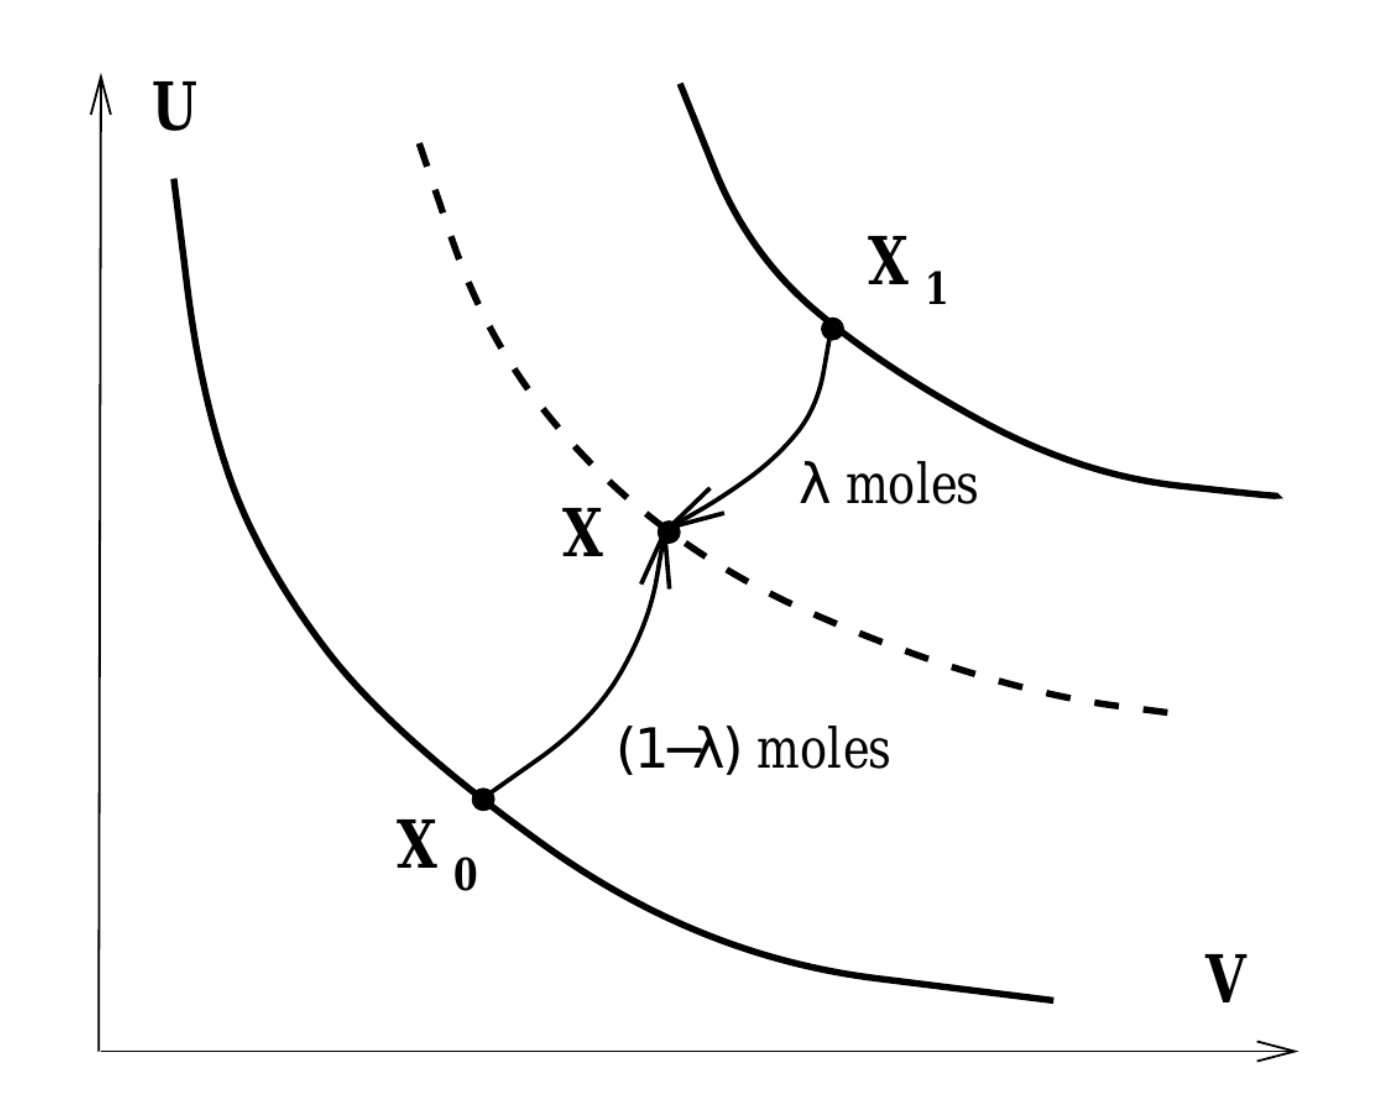
\includegraphics[width=50mm]{fig2.png}
    \end{center}
    \caption{カノニカルエントロピー}
    \label{fig:one}
\end{figure}
Lemma2.1により、カノニカルエントロピーは、well-definedであり、$S_{\Gamma}(X)<\infty$である。\\

\begin{itembox}[l]{\textbf{Lem2.2:$\prec$と$\leq$の関係}}
    いま、$X_0 \prec \prec X_1$であるとし、$a_0,a_1,a_0',a_1' \in \mathbb{R}$に対して、$a_0+a_1=a_0'+a_1'$であるとする。このとき、\\
    (1)$((a_0X_0,a_1X_1) \prec (a_0'X_0,a_1'X_1))$\\
    (2)$ a_1 \leq a_1' $(ゆえに、$a_0 \leq a_0'$)\\
    は同値である。\\
    特に、もし、$a_1=a_1',a_0=a_0'$であるならば、(1)の$\prec$は$\overset{A}{\sim}$に置き換えることができる。
\end{itembox}
これは、例えば、温度の高い系と低い系を接触させたときに、エントロピーが増加することを示している。\\
\textbf{Prf}\\
ここでは、$a_0,a_1,a_0',a_1'$が全て正であり、$a_0+a_1=a_0'+a_1'=1$であるとする。また、$a_1=\lambda,a_1'=\lambda'$とする。\\
(1)$\Rightarrow$(2)\\
背理法により示す。すなわち、$\lambda > \lambda'$とする。今、
\begin{equation}
    ((1-\lambda)X_0,\lambda X_1) \prec ((1-\lambda')X_0',\lambda'X_1')
\end{equation}
ここで、
\begin{align}
    ((1-\lambda)X_0,\lambda X_1) &\overset{A}{\sim} ((1-\lambda)X_0,\lambda'X_1,(\lambda-\lambda')X_1)\\
    ((1-\lambda')X_0,\lambda'X_1') &\overset{A}{\sim} ((1-\lambda)X_0,(\lambda - \lambda')X_0,\lambda'X_1)
\end{align}
であるから、
\begin{equation}
    ((1-\lambda)X_0,\lambda'X_1,(\lambda-\lambda')X_1) \prec ((1-\lambda)X_0,(\lambda - \lambda')X_0,\lambda'X_1)
\end{equation}
である。ここで、キャンセル法則を用いると、
\begin{equation}
    (\lambda - \lambda')X_1 \prec (\lambda - \lambda')X_0
\end{equation}
$\lambda -\lambda '>0$と、スケーリング不変性より、
\begin{equation}
    X_1 \prec X_0
\end{equation}
であるが、これは、$X_0 \prec \prec X_1$に矛盾する。\\
(2)$\Rightarrow$(1)\\
\begin{align}
    ((1-\lambda)X_0,\lambda X_1) &\overset{A}{\sim} ((1-\lambda')X_0,(\lambda'-\lambda)X_0,\lambda X_1)\\
    &\prec ((1-\lambda')X_0,(\lambda'-\lambda)X_1,\lambda X_1)\\
    &\overset{A}{\sim} ((1-\lambda')X_0,\lambda'X_1)
\end{align}
であるから、(1)が示された。 \hfill\qedsymbol\\


\begin{itembox}[l]{\textbf{Lem2.3:エントロピーの特徴づけ}}
$S_{\Gamma}$が、$\Gamma$上のカノニカルエントロピーであるとし、基準点を$X_0 \prec \prec X_1$とする。もし、$X\in \Gamma$であるならば、
\begin{equation}
    \lambda = S_{\Gamma}(X)
\end{equation}
は、
\begin{equation}
    X \overset{A}{\sim} ((1-\lambda)X_0,\lambda X_1)
\end{equation}
と同値である。\\

\end{itembox}
\textbf{Prf}\\
((53)$\Rightarrow$(54))\\
$\lambda = S_{\Gamma}(X)$とする。このとき、supの定義より、0に収束する列$\epsilon_n$の列が存在して、
\begin{equation}
    ((1-(\lambda-\epsilon_n))X_0,(\lambda-\epsilon_n)X_1) \prec X
\end{equation}
である。任意のnについて、
\begin{align}
    ((1-\lambda)X_0,\lambda X_1,\epsilon_n X_0) &\overset{A}{\sim} ((1-(\lambda+\epsilon_n))X_0,(\lambda-\epsilon_n)X_1,\epsilon_n X_1)\\
    &\prec (X,\epsilon_n X_1)
\end{align}
である。安定性を用いて、
\begin{equation}
    ((1-\lambda)X_0,\lambda X_1) \prec X
\end{equation}
である。\\
また、$\lambda$はsupなので、
\begin{equation}
    X \prec ((1-(\lambda+\epsilon))X_0,(\lambda+\epsilon)X_1)
\end{equation}
である。変形して、
\begin{equation}
    X+\epsilon X_0 \prec ((1-\lambda)X_0,\lambda X_1)
\end{equation}
である。ここで、安定性を用いて、
\begin{equation}
    X \prec ((1-\lambda)X_0,\lambda X_1)
\end{equation}
以上より、
\begin{equation}
    X \overset{A}{\sim} ((1-\lambda)X_0,\lambda X_1)
\end{equation}
である。 \\

((54)$\Rightarrow$(53))\\

\textbf{Prf(Thm2.2)}\\
((1)$\Rightarrow$(2))\\
$\lambda_i = S_{\Gamma}(Y_i)$とする。このとき、Lem2.3より、
\begin{align}
    Y_i \overset{A}{\sim} (1-S_{\Gamma}(Y_i))X_0,S_{\Gamma}(Y_i)X_1\\
    Y_i' \overset{A}{\sim} (1-S_{\Gamma}(Y_i'))X_0,S_{\Gamma}(Y_i')X_1
\end{align}
である。これより、
\begin{align}
    (t_1 Y_1,t_2 Y_2,\cdots,t_n Y_n) &\overset{A}{\sim} (\sum_{i=1}^n t_i(1-S_{\Gamma}(Y_i))X_0,\sum_{i=1}^n t_i S_{\Gamma}(Y_i)X_1)\\
    (t_1' Y_1',t_2' Y_2',\cdots,t_n' Y_n') &\overset{A}{\sim} (\sum_{i=1}^n t_i'(1-S_{\Gamma}(Y_i'))X_0,\sum_{i=1}^n t_i' S_{\Gamma}(Y_i')X_1)
\end{align}
である。ここで、右辺について、Lem2.2より、
\begin{equation}
    \sum_{i=1}^n t_i S_{\Gamma}(Y_i) \leq \sum_{i=1}^n t_i' S_{\Gamma}(Y_i')
\end{equation}
である。\\
((2)$\Rightarrow$(1))\\
略。(要するに、普段扱っているエントロピーが自然な仮説$A_1-A_6$およびCHを満たすか確かめる作業である。)\\
以上より、示された。\hfill\qedsymbol\\

\begin{itembox}[l]{\textbf{Thm:エントロピーの一意性}}
もし、$S_{\Gamma}^*$が、任意の$\lambda \in \mathbb{R}$と、$X,Y,X',Y' \in \Gamma $に対して、
\begin{align}
    ((1-\lambda)X,\lambda Y) &\prec ((1-\lambda')X',\lambda' Y') \\
    \Leftrightarrow (1-\lambda)S_{\Gamma}^*(X)+\lambda S_{\Gamma}^*(Y) &\leq (1-\lambda')S_{\Gamma}^*(X')+\lambda' S_{\Gamma}^*(Y')
\end{align}
であるならば、
\begin{equation}
    S_{\Gamma}^*(X)=aS_{\Gamma} (X)+b
\end{equation}
で表される。ただし、
\begin{align}
    a = S_{\Gamma}^*(X_1)-S_{\Gamma}^*(X_0)>0\\
    b = S_{\Gamma}^*(X_0)
\end{align}
である。\\
ここで、$S_{\Gamma}$は、$\Gamma$上のカノニカルエントロピーで、参照点は$X_0 \prec \prec X_1$である。
\end{itembox}
\textbf{Prf}\\
Lem2.3より、
\begin{equation}
    X \overset{A}{\sim} ((1-\lambda)X,\lambda X) \overset{A}{\sim} ((1-\lambda')X_0,\lambda' X_1)
\end{equation}
である。$S_{\Gamma}^*$に関する仮定(Thm2.2)より、
\begin{equation}
    S_{\Gamma}^*(X) = (1-\lambda')S_{\Gamma}^*(X_0)+\lambda' S_{\Gamma}^*(X_1)=(S_{\Gamma}^*(X_1)-S_{\Gamma}^*(X_0))\lambda'+S_{\Gamma}^*(X_0)
\end{equation}
ここで、$X \overset{A}{\sim} ((1-\lambda')X_0,\lambda' X_1)$であるから、Lem2.3より、$\lambda ' = S_{\Gamma}(X)$である。\\
以上より、
\begin{equation}
    S_{\Gamma}^*(X) = aS_{\Gamma}(X)+b
\end{equation}
である。\hfill\qedsymbol\\

カノニカルエントロピーの定義をみてみると、エントロピーは、二重スケール積$\Gamma(1-\lambda)\times \Gamma(\lambda)$上の関係$\prec$と、基準点$X_0 \prec \prec X_1$のみに依存している。\\
さらに、エントロピー原理の定式化を見てみると、エントロピーは、すべての複数スケールコピー上での関係を特徴づける。すなわち、CHがすべての複数スケールコピーにおいて成立することを示している。\\
以上を踏まえると、Thm2.3は以下のように書き換えることができる。\\

\begin{itembox}[l]{\textbf{Thm:エントロピーの一意性(2)}}
    $\prec$と$\prec ^*$を、$\Gamma$上のスケールコピーにおける関係とし、公理A1-A6を満たし、さらに、固定された各$\lambda \in [0,1]$について、$\Gamma(1-\lambda)\times \Gamma(\lambda)$についてCHも満たすとする。\\
    もし、$\prec$と$\prec ^*$が[0,1]の各$\lambda\in [0,1]$について、$\Gamma(1-\lambda)\times \Gamma(\lambda)$上で一致しているならば、$\prec$と$\prec ^*$は$\Gamma$のすべての複数スケールコピー上で一致し、CHはすべての複数スケールコピーにおいて成立する。
\end{itembox}

\section{普遍的なエントロピーの構成}
\begin{itembox}[l]{\textbf{Def:エントロピー定数}}
    Thm2.3における$a,b$を、エントロピー定数という。
\end{itembox}
我々の目標は、これらのエントロピーをまとめて、さまざまな系の任意の多重スケーリングコピー積に対して正しく振舞うことを示すことである。\\
また、この普遍的エントロピーは、系ごとに乗法定数が一意に定まる。\\
ここでの問題は、キャリブレーションである。すなわち、各基本エントロピーの前にある乗法定数を、(2.4)が守られるように選択する必要がある。\\
このsectionでは、以下の定理を証明する。これは、Thm2.2の一般化である。\\

\begin{itembox}[l]{\textbf{Thm:Consistent entropy scales}}
以下の要件を満たす系からなる族(SF)を考える。\\
\begin{itemize}
    \item[(1)] SFの任意の二つの系の状態空間は互いに素な集合である。すなわち、SF内のすべての状態はちょうど一つの状態空間に属する。\\
    \item[(2)] SF内の任意の多重スケーリング積もまたSFに属する。\footnote{ただし、例えば$\Gamma_1 \times \Gamma_2$は$\Gamma_1$や$\Gamma_2$と互いに素である。}\\
    \item[(3)] SF内の任意の系がCHを満たす。\\
\end{itemize}
それぞれの状態空間$\Gamma$に対して、$S_{\Gamma}$を$\Gamma$上ある確定されたエントロピー関数とする。このとき、$\Gamma$のすべての状態に対して定義される関数
\begin{equation}
    S(X) = a_{\Gamma}S_{\Gamma}(X)+b_{\Gamma} \quad X \in \Gamma
\end{equation}
が、以下の性質を持つ。\\
\begin{itemize}
    \item[(a)] もし、$X$と$Y$が同じ状態空間に属するならば、$X \prec Y \Leftrightarrow S(X) \leq S(Y)$である。\\
    \item[(b)] $S$は相加性と示量性を持つ。すなわち、
    \begin{align}
        S(X,Y) &= S(X)+S(Y)\\
        S(tX) &= tS(X)
    \end{align}
    である。\\
\end{itemize}
\end{itembox}
\textbf{Prf}\\
ある系$\Gamma_0$と、$\Gamma_0$上の二点$Z_0 \prec \prec Z_1$を選ぶ。それのれの状態空間に対して、ある固定点$X_{\Gamma}\in \Gamma$を、
\begin{align}
    X_{\Gamma_1 \times \Gamma_2} &= (X_{\Gamma_1},X_{\Gamma_2})\\
    X_{t\Gamma} &= tX_{\Gamma}
\end{align}
が成り立つように選ぶ。\\
中略\\
$X \in \Gamma$に対して、$\Gamma \times \Gamma_0$とその空間上の、基準点が$(X_{\Gamma},Z_0),(X_{\Gamma},Z_1)$であるようなカノニカルエントロピーを考える。このとき、新たにエントロピー関数を、
\begin{equation}
    S(X)=S_{\Gamma_1 \times \Gamma_2}((X,Z_0)|(X_{\Gamma},Z_0),(X_{\Gamma},Z_1))
\end{equation}
と定義する。\\
このように定義すると、合成系について、Le.2.3を適用することで、
\begin{equation}
    (X,Z_0) \overset{A}{\sim} ((1-\lambda)(X_{\Gamma},Z_0),\lambda(X_{\Gamma},Z_1))
\end{equation}
である。ただし、$\lambda = S(X)$である。これを変形することにより、
\begin{equation}
    (X,\lambda Z_0) \overset{A}{\sim} (X_{\Gamma},\lambda Z_1)
\end{equation}
である。この(83)式を整理することで、エントロピーの加法性を示すことができる。\\
\textbf{加法性}\\
\begin{align}
    (X_1,\lambda_1 Z_0) &\overset{A}{\sim} (X_{\Gamma_1},\lambda_1 Z_1)\\
    (X_2,\lambda_2 Z_0) &\overset{A}{\sim} (X_{\Gamma_2},\lambda_2 Z_1)\\
    (X,\lambda Z_0) &\overset{A}{\sim} (X_{\Gamma},\lambda Z_1)
\end{align}
である。上二つの式から、
\begin{align}
    ((X_1,\lambda_1 Z_0),(X_2,\lambda_2 Z_0)) &\overset{A}{\sim} ((X_{\Gamma_1},\lambda_1 Z_1),(X_{\Gamma_2},\lambda_2 Z_1))\\
    &\overset{A}{\sim} (X_{\Gamma_1},X_{\Gamma_2},(\lambda_1+\lambda_2)Z_1)
\end{align}
である。これと(86)式を比較して、
\begin{equation}
    S(X_1)+S(X_2) = S(X_1,X_2)
\end{equation}
である。\\
\textbf{示量性}\\
\begin{align}
    (X,\lambda Z_0) &\overset{A}{\sim} (X_{\Gamma},\lambda Z_1)\\
    (tX,\lambda' Z_0) &\overset{A}{\sim} (X_{t\Gamma},\lambda' Z_1)=(tX_{\Gamma},\lambda' Z_1)\\
    (tX,\lambda' Z_0) &\overset{A}{\sim} (X_{\Gamma},\frac{\lambda'}{t} Z_1)
\end{align}
であるから、
\begin{equation}
    \lambda = \frac{\lambda'}{t}
\end{equation}
であるから、$S(tX)=tS(X)$である。\\
また、これがエントロピーとしての資格を持つことは、以下のように示すことができる。\\
\textbf{エントロピー増大則}\\
\begin{equation}
    X \prec Y \Leftarrow S(X) \leq S(Y)
\end{equation}
を示す。キャンセル法則を用いることにより、
\begin{equation}
    X \prec Y \Leftarrow (X,Z_0) \prec (Y,Z_0)
\end{equation}
である。また、Thm2.2により、
\begin{equation}
    (X,Z_0) \prec (Y,Z_0) \Leftrightarrow S(X,Z_0) \leq S(Y,Z_0) \Leftrightarrow S(X) \leq S(Y)
\end{equation}
であるから、エントロピー増大則が示された。\hfill\qedsymbol\\

\begin{itembox}[l]{\textbf{Def:一貫したエントロピー}}
    状態空間$\Gamma$上のエントロピー関数$S_{\Gamma}$が一貫したエントロピーであるとは、$\Gamma$上のエントロピー関数の適切な線形結合が、任意の多重スケーリング積のエントロピー関数として働くことである。\\
    すなわち、$a_{\Gamma}$を1にとることができるということである。

\end{itembox}

\textbf{注意}\\
エントロピー関数は、
\begin{equation}
    S(X) =sup\{\lambda|(X_{\Gamma},\lambda Z_1)\prec (X,\lambda Z_0)\}
\end{equation}
とも書くことができる。\\

\section{エントロピーの凸性}
\begin{itembox}[l]{\textbf{Def:凸な状態空間}}
    状態空間$\Gamma$が凸であるとは、任意の$X,Y \in \Gamma$について、
    \begin{equation}
        (tX+(1-t)Y) \in \Gamma \quad (0 \leq t \leq 1)
    \end{equation}
    が成立することである。
\end{itembox}

さて、以上の定義のもと、断熱到達可能性に、以下の公理を追加する。\\
\begin{itembox}[l]{\textbf{順序関係の公理A7}}
    状態空間$\Gamma$が凸であるとし、$X,Y \in \Gamma$であるとする。このとき、
    \begin{equation}
        (tX,(1-t)Y) \prec tX+(1-t)Y
    \end{equation}
    が成立する。
\end{itembox}
この要請の物理的要請は、独立した二つの系を合成したとき、例えばエネルギーや体積が加算されることを意味する。

\begin{itembox}[l]{\textbf{Def:forward sector}}
    状態空間$\Gamma,\Gamma'$と、$X \in \Gamma,Y \in \Gamma'$に対して、
    \begin{equation}
        A_X = \{Y \in \Gamma'|X \prec Y\}
    \end{equation}
    を、$X$のforward sectorという。
\end{itembox}
\begin{itembox}[l]{\textbf{Thm:forward sectorの凸性}}
    $\Gamma,\Gamma'$を状態空間とし、$\Gamma '$が凸であるとする。このとき、$X \in \Gamma$に対して、$A_X$は$\Gamma'$の凸集合である。
\end{itembox}
\textbf{Prf}\\
$X \prec Y_1,Y_2$であるとし、$0 < t < 1$とする。このとき、
\begin{align}
    X \prec tY_1+(1-t)Y_2
\end{align}
を示せばよい。A5より、
\begin{equation}
    X \prec (tX,(1-t)X)
\end{equation}
である。また、$X \prec Y_1,Y_2$であるから、
\begin{align}
    (tX,(1-t)X) \prec (tY_1,(1-t)Y_2)
\end{align}
である。これと、A7より、
\begin{equation}
    X \prec tY_1+(1-t)Y_2
\end{equation}
である。以上より、示された。\hfill\qedsymbol\\
とくに、同じ状態空間内でのA7と上の定理を図示すると、以下のようになる。\\
\begin{figure}[H]
    \begin{center}
    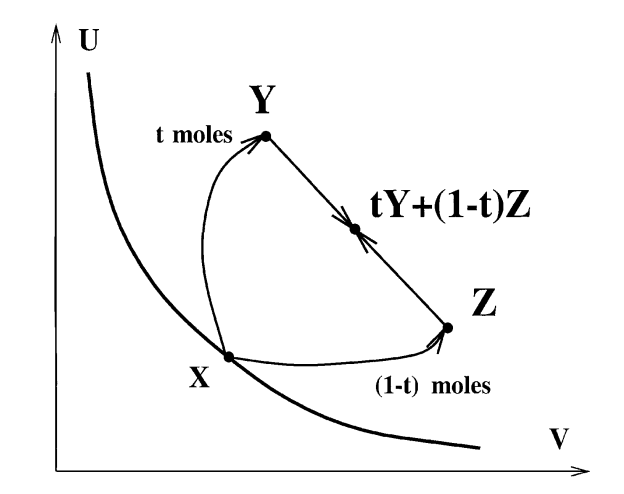
\includegraphics[width=100mm]{fig3.png}
    \end{center}
    \caption{forward sector}
    \label{fig:two}
\end{figure}
すなわち、断熱到達可能なYとZが存在するとき、YとZの間には、さらに断熱到達可能な点が存在するということである。\\

\begin{itembox}[l]{\textbf{Thm:$\mathcal{S}_{\lambda}$の凸性}}
    状態空間$\Gamma$が凸であるとき、以下の二つが成立する。
    \begin{itemize}
        \item[(1)] $\mathcal{S}_{\lambda}$は、$\Gamma$の凸集合である。
        \item[(2)] もし、$X \in \mathcal{S}_{\lambda}$であり、$0 \leq t \leq 1$であるならば、$tX + (1-t)Y \in \mathcal{S}_{t\lambda \times (1-t)\lambda}$である。
    \end{itemize}
\end{itembox}
\textbf{Recall}\\
$\mathcal{S}_{\lambda}= \{X \in \Gamma|((1-\lambda)X_0,\lambda X_1) \prec X\}$である。\\
\textbf{Prf}\\
(1)\\
$X,Y \in \mathcal{S}_{\lambda}$であるとする。このとき、
\begin{align}
    tX+(1-t)Y \in \mathcal{S}_{\lambda}
\end{align}
を示せばよい。ここで、$X,Y \in \mathcal{S}_{\lambda}$であるから、
\begin{align}
    ((1-\lambda)X_0,\lambda X_1) &\prec X\\
    ((1-\lambda)X_0,\lambda X_1) &\prec Y
\end{align}
である。したがって、
\begin{align}
    t((1-\lambda)X_0,\lambda X_1) &\prec tX\\
    (1-t)((1-\lambda)X_0,\lambda X_1) &\prec (1-t)Y
\end{align}
である。したがって、
\begin{align}
    t((1-\lambda)X_0,\lambda X_1)+(1-t)((1-\lambda)X_0,\lambda X_1) &\prec tX+(1-t)Y\\
    ((1-\lambda)X_0,\lambda X_1) &\prec tX+(1-t)Y
\end{align}
である。以上より、(1)が示された。\\
(2)\\
後で書く。\\

\begin{itembox}[l]{\textbf{Thm:エントロピーの凸性}}
    状態空間$\Gamma$が凸であるとする。このとき、エントロピー関数$S_{\Gamma}$は、
    \begin{equation}
        S_{\Gamma}(tX+(1-t)Y) \geq tS_{\Gamma}(X)+(1-t)S_{\Gamma}(Y)
    \end{equation}
    である。すなわち、$S_{\Gamma}$は、上に凸である。
\end{itembox}
\textbf{Prf}\\
$X \in \mathcal{S}_{\lambda_1},Y \in \mathcal{S}_{\lambda_2}$であるとする。このとき、Thm2.7より、
\begin{align}
    tX+(1-t)Y \in \mathcal{S}_{t\lambda_1+(1-t)\lambda_2}
\end{align}
である。このとき、エントロピーの定義から、
\begin{align}
    S_{\Gamma}(tX+(1-t)Y) &\geq t\lambda_1+(1-t)\lambda_2\\
\end{align}
である。したがって、右辺の$\lambda_1,\lambda_2$についてsupを取ることにより、
\begin{align}
    S_{\Gamma}(tX+(1-t)Y) &\geq tS_{\Gamma}(X)+(1-t)S_{\Gamma}(Y)
\end{align}
である。以上より、示された。\hfill\qedsymbol\\

\section{不可逆過程とカラテオドリの原理}
\begin{itembox}[l]{\textbf{Thm:カラテオドリの原理と不可逆過程}}
    状態空間$\Gamma$が凸であり、$\mathbb{R}^n$の部分空間であるとする。このとき、以下の二つの主張を考える。
    \begin{itemize}
        \item[(1)] 不可逆過程の存在:任意の$X \in \Gamma$に対して、$X \prec \prec Y$となる$Y \in \Gamma$が存在する。
        \item[(2)] カラテオドリの原理:任意の$X \in \Gamma$の任意の近傍にたいして、$Z \overset{A}{\sim} X$が偽となる$Z \in \Gamma$が存在する。 
    \end{itemize}
    このとき、(1)$\Rightarrow$(2)である。\\
また、$\Gamma$上の任意のforward sectorが、成分0をもたないならば、(2)$\Rightarrow$(1)である。
\end{itembox}
\textbf{Prf}\\
一旦省略\\




\end{document}
